\documentclass{article}

\usepackage{fullpage}
\usepackage{tabularx}
\usepackage{booktabs}
\usepackage{setspace}
\doublespacing

\usepackage{float}


\newcommand{\pkg}[1]{\texttt{#1}}
\newcommand{\cmd}[1]{\texttt{#1}}
\newcommand{\prog}[1]{{\sf #1}}
\newcommand{\proglang}[1]{\prog{#1}}
\newcommand{\R}{\prog{R}}

\usepackage{longtable}
\usepackage{pdflscape}
\usepackage[T1]{fontenc}
\usepackage{listings}
\usepackage{color}
\definecolor{lightgray}{rgb}{.9,.9,.9}
\definecolor{darkgray}{rgb}{.4,.4,.4}
\definecolor{purple}{rgb}{0.65, 0.12, 0.82}

\lstdefinelanguage{JavaScript}{
  keywords={typeof, new, true, false, catch, function, return, null, catch, switch, var, if, in, while, do, else, case, break},
  keywordstyle=\color{blue}\bfseries,
  ndkeywords={class, export, boolean, throw, implements, import, this},
  ndkeywordstyle=\color{darkgray}\bfseries,
  identifierstyle=\color{black},
  sensitive=false,
  comment=[l]{//},
  morecomment=[s]{/*}{*/},
  commentstyle=\color{purple}\ttfamily,
  % stringstyle=\color{orange}\ttfamily,
  morestring=[b]',
  morestring=[b]"
}

\lstset{
   language=JavaScript,
   % backgroundcolor=\color{lightgray},
   extendedchars=true,
   basicstyle=\footnotesize\ttfamily,
   showstringspaces=false,
   showspaces=false,
   numbers=left,
   numberstyle=\footnotesize,
   numbersep=9pt,
   tabsize=2,
   breaklines=true,
   showtabs=false,
   captionpos=b,
   upquote=true
}

\usepackage[
    backend=biber,
    style=apa,
    sorting=nty
]{biblatex}
\addbibresource{references.bib}

\usepackage{authblk}
\usepackage{graphicx} % Required for inserting images
\usepackage[acronym]{glossaries}
% \usepackage[automake]{glossaries-extra}

\makeglossaries
\newacronym{iife}{IIFE}{instantaneously invoked function expression}
\newacronym{api}{API}{application programming interface}
\newacronym{gui}{GUI}{graphical user interface}
\newacronym{ux}{ux}{user experience}


\title{A review of interactive graphics for data exploration and analysis}
\author{Tom Elliott}
\affil{\small iNZight Analytics Ltd\\
Iwi affiliations: Ngāti Whakaue, Ngāti Raukawa}

\date{}

\begin{document}

\maketitle

\begin{abstract}
Interactive data visualization has become fundamental to modern data analysis, enabling deeper insights and more intuitive exploration of complex datasets. This paper reviews the evolution and current state of interactive graphics for data exploration and analysis, with particular focus on R-based tools and web technologies. We examine existing frameworks and tools, discussing their strengths and limitations in facilitating interactive data analysis. Building on this review, we propose a new ecosystem that leverages R and web technologies to create privacy-preserving interactive visualization tools, addressing key challenges in secure data access and analysis. Our proposed framework emphasizes the separation of front-end visualization from back-end data processing, enabling fine-grained access control while maintaining rich interactive capabilities for data exploration and statistical analysis.
\end{abstract}

\section{Introduction}
\label{sec:intro}

Data visualization has become an essential component of modern data analysis, transforming how we understand and interpret complex datasets. The ability to interactively explore data through visual representations has revolutionized the analytical process, enabling researchers and analysts to uncover patterns, identify relationships, and generate insights more effectively than ever before.

Over the past decades, visualization tools have evolved significantly, shifting from static desktop applications to dynamic web-based platforms. This evolution has been particularly notable in the R ecosystem, which has developed a rich collection of packages for data visualization and analysis. While traditional statistical graphics remain valuable, the emergence of interactive visualization tools has opened new possibilities for data exploration and analysis.

The landscape of data visualization tools spans from specialized applications addressing specific analytical needs to broader platforms leveraging modern web technologies. As highlighted by \cite{Cook2007}, \cite{Theus2014}, and \cite{Ward2015}, interactive visualization plays a crucial role in the modern data analysis process. However, while many existing tools offer interactive capabilities, there remains a need for solutions that effectively balance accessibility, security, and analytical power.

This review examines the current state of interactive graphics for data exploration and analysis, with particular attention to tools and frameworks based on R and web technologies. We focus on solutions that can be readily reproduced and extended, addressing the growing need for secure, scalable data visualization platforms.

\section{Evolution of Interactive Graphics}
\label{sec:evolution}

The development of interactive graphics has been shaped by advances in both statistical methodology and computing technology. Early systems were limited by computational power and display capabilities, but modern web technologies have removed many of these constraints, enabling more sophisticated and responsive visualizations.

Traditional statistical graphics focused on static representations, requiring analysts to create multiple views to understand different aspects of their data. The advent of interactive graphics transformed this paradigm by allowing direct manipulation of visualizations, enabling users to explore different perspectives of their data dynamically. This shift has been particularly important in exploratory data analysis, where the ability to quickly generate and modify visualizations is crucial.

The rise of web technologies has further accelerated this evolution, making interactive graphics more accessible and easier to distribute. Modern browsers now support sophisticated visualization capabilities through technologies like SVG, Canvas, and WebGL, while JavaScript libraries such as D3.js have become standard tools for creating interactive visualizations.

\section{Interactive Graphics for Data Analysis}
\label{sec:interactive-graphics}

In the context of data analysis, interactive graphics serve as both exploratory tools and interfaces for statistical computation. An interactive graphic is one that allows users to interact with the data through the graphic as a \gls{ui} \parencite{Young2011}. This interaction can take many forms, from simple hover effects to complex linked views and statistical computations.

Key features of modern interactive graphics include:

\begin{itemize}
\item \textbf{Direct Manipulation:} Users can interact directly with visual elements through brushing, selecting, and dragging operations. Brushing, particularly, allows users to select subsets of data points by dragging the mouse over the graphic.

\item \textbf{Linked Views:} Multiple graphics can be coordinated so that interactions with one view are reflected in others. This linking enables users to explore relationships between different aspects of their data simultaneously.

\item \textbf{Dynamic Updates:} Graphics can update in real-time in response to user actions, including filtering, aggregation, and statistical computations.

\item \textbf{Context-Sensitive Operations:} Context menus and tool panels provide access to relevant operations based on the current selection or view.
\end{itemize}

Existing systems demonstrate various approaches to implementing these features. \proglang{Mondrian} \parencite{Theus2014} provides a menu-driven interface for creating linked views, while \proglang{ViSta} \parencite{Young1996,Young2011} offers pre-defined sets of linked graphics (SpreadPlots) for specific analytical tasks. More recent developments like \proglang{plotscaper} \cite{Bartonicek2024} leverage modern web technologies to create interactive linked graphics with emphasis on statistical summaries.

\section{Interactive Data Analysis Process}
\label{sec:interactive-data-analysis}

Interactive data analysis extends beyond mere visualization to encompass the entire analytical workflow. This process involves iterative exploration, model fitting, and result interpretation, all supported by interactive tools. The key aspects of this process include:

\begin{itemize}
\item \textbf{Exploratory Data Analysis:} Interactive visualization enables rapid exploration of data distributions, relationships, and potential patterns.

\item \textbf{Model Building:} Visual interfaces can guide the model-building process, allowing users to fit and compare different models interactively.

\item \textbf{Result Interpretation:} Interactive graphics help in understanding model results and checking assumptions through diagnostic plots and visual summaries.

\item \textbf{Communication:} Interactive visualizations serve as effective tools for communicating findings to different audiences.
\end{itemize}

The integration of these aspects requires careful consideration of both technical implementation and user interface design. Systems must balance flexibility with ease of use, providing sophisticated analytical capabilities while maintaining an intuitive interface.

\section{Proposed Framework}
\label{sec:framework}

Building on our review of existing tools and current needs, we propose a new framework for interactive graphics that addresses several key challenges in modern data analysis. Our framework is based on a client-server architecture using R and web technologies, specifically leveraging the Rserve ecosystem.

\subsection{Architecture}
The proposed system separates concerns between front-end visualization and back-end computation, offering several advantages:

\begin{itemize}
\item \textbf{Security:} Fine-grained access control at the server level ensures data privacy while enabling rich interactive capabilities.

\item \textbf{Scalability:} Server-side processing allows handling of large datasets without client-side performance issues.

\item \textbf{Flexibility:} The separation of concerns enables independent evolution of visualization and computational components.
\end{itemize}

\begin{figure}[H]
    \centering
    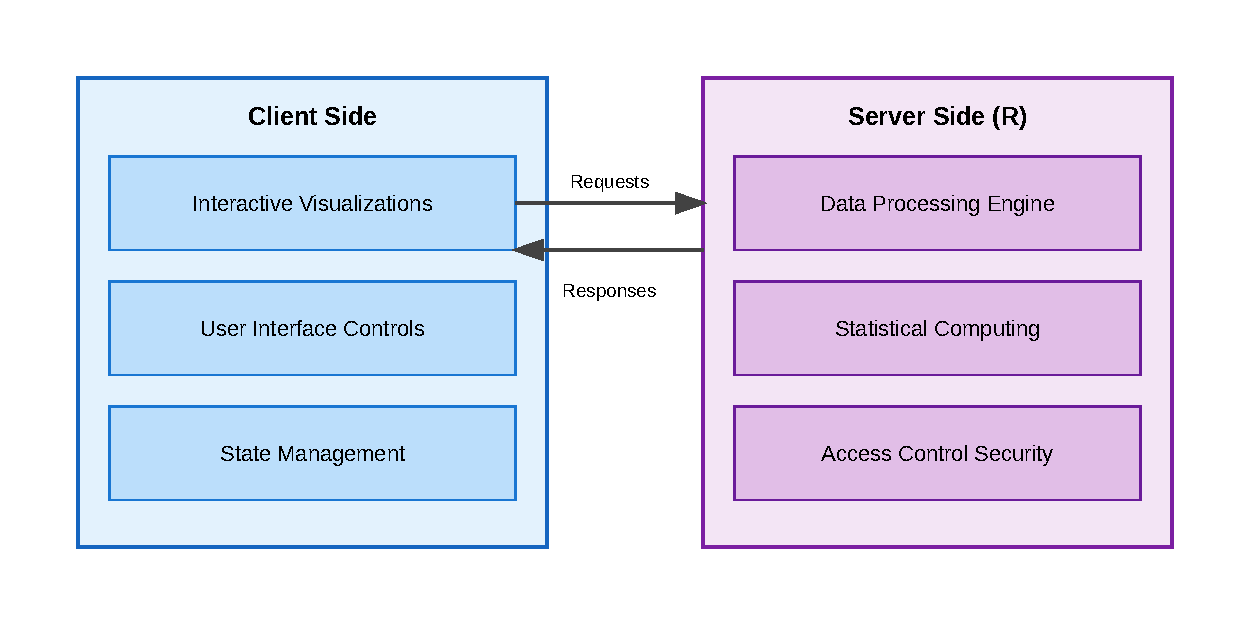
\includegraphics[width=0.9\textwidth]{system-architecture.pdf}
    \caption{High-level system architecture showing the separation between client and server components.}
    \label{fig:system-architecture}
\end{figure}

\subsection{Key Features}
Our proposed framework includes several innovative features:

\begin{itemize}
\item \textbf{Server-Side Linking:} Graphics are linked through server-side state management, ensuring consistency and enabling privacy-preserving interactions.

\item \textbf{Dynamic Computation:} Statistical summaries and visualizations are computed on-demand, allowing for real-time analysis of large datasets.

\item \textbf{Access Control:} Fine-grained permissions ensure users can only access appropriate data and analyses.

\item \textbf{Result Sharing:} Secure sharing mechanisms allow collaboration while maintaining access controls.
\end{itemize}

\begin{figure}[H]
    \centering
    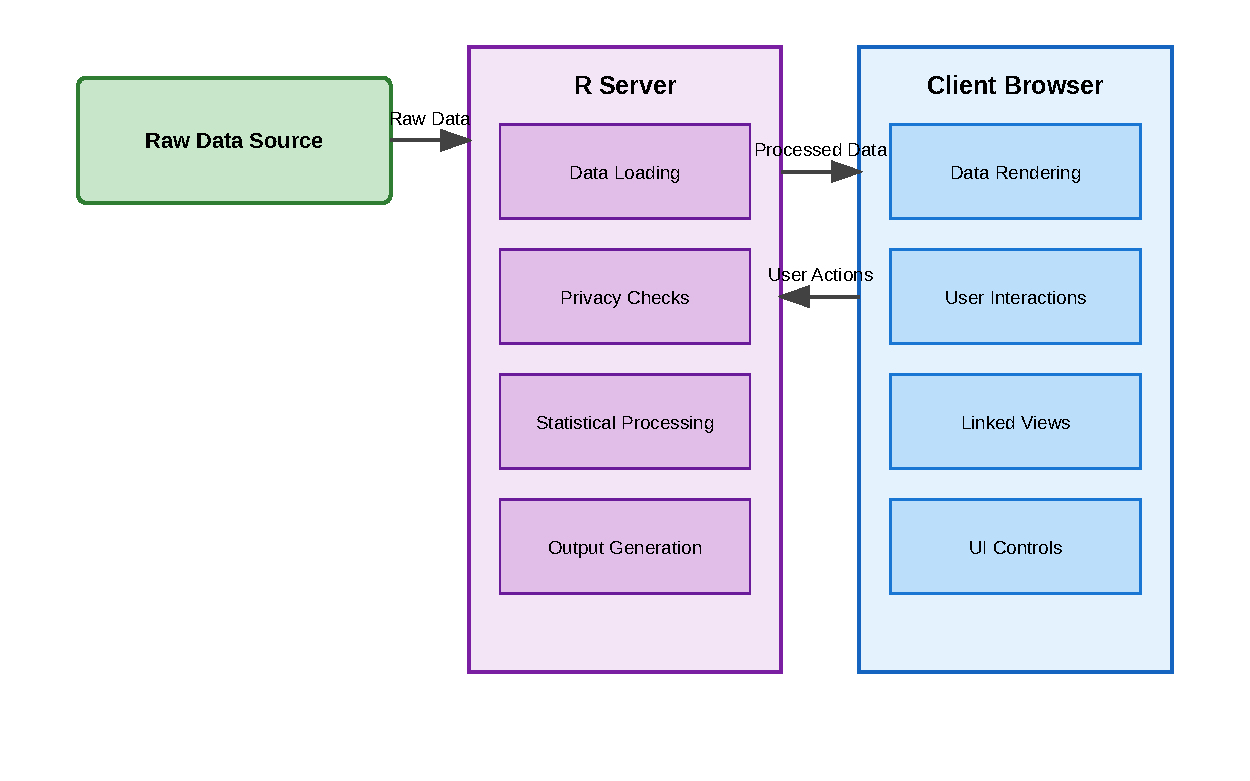
\includegraphics[width=0.9\textwidth]{data-flow.pdf}
    \caption{Data flow and interaction between system components.}
    \label{fig:data-flow}
\end{figure}

\subsection{Implementation Considerations}
The implementation of this framework requires careful attention to several aspects:

\begin{itemize}
\item \textbf{Data Transfer:} Efficient protocols for transmitting data between server and client while maintaining privacy.

\item \textbf{State Management:} Robust handling of user sessions and visualization state.

\item \textbf{Caching:} Strategic caching of results to balance responsiveness with real-time computation.
\end{itemize}


\section{Future Directions}
\label{sec:future}

The proposed framework opens several avenues for future development:

\begin{itemize}
\item \textbf{Extended Visualization Types:} Development of new interactive visualization types specifically designed for privacy-preserving analysis.

\item \textbf{Advanced Statistical Methods:} Integration of more sophisticated statistical methods while maintaining interactive capabilities.

\item \textbf{Collaborative Features:} Enhanced support for collaborative analysis while maintaining security constraints.
\end{itemize}

\section{Conclusion}
\label{sec:conclusion}

Interactive graphics have become essential tools in modern data analysis, enabling more intuitive and effective exploration of complex datasets. Our proposed framework builds on existing work to address current challenges in secure, scalable data analysis. By separating front-end visualization from back-end computation, we enable sophisticated interactive analysis while maintaining data privacy and security.

The framework we propose represents a step toward more accessible and secure data analysis tools, particularly valuable for organizations dealing with sensitive data. Future work will focus on expanding the capabilities of this system while maintaining its core principles of security, scalability, and usability.

\section*{Acknowledgements}

Supported by the Ngā Puanga Pūtaiao Fellowships from Government funding, administered by the Royal Society Te Apārangi.

\printglossary[type=\acronymtype,nonumberlist,nopostdot]

\printbibliography

\end{document}
